\chapter{Related work}
\label{cha2}

This chapter gives an overview of the relative research areas: robot grasping and manipulation, imitation learning and modular approaches. In Section \ref{cha2:sec1:grasping} we overview the studies in robot grasping and manipulation, outline the current challenges in the area. In Section \ref{cha2:sec2:learning}, we introduce the technique of robot imitation learning (program by demonstration) and particularly look at its applications in robot grasping and manipulation. In Section \ref{cha2:sec3:modular} we first discuss the motivation of modular approaches and its biological inspiration. We then give a brief review on modular approaches in control theory (multiple module adaptive control). The final part of this section focus on the applications of modular approaches in robotics, especially in grasping and manipulation. Figure \ref{fig:litreview} depict the structure of this section.

\begin{figure}
\centering
  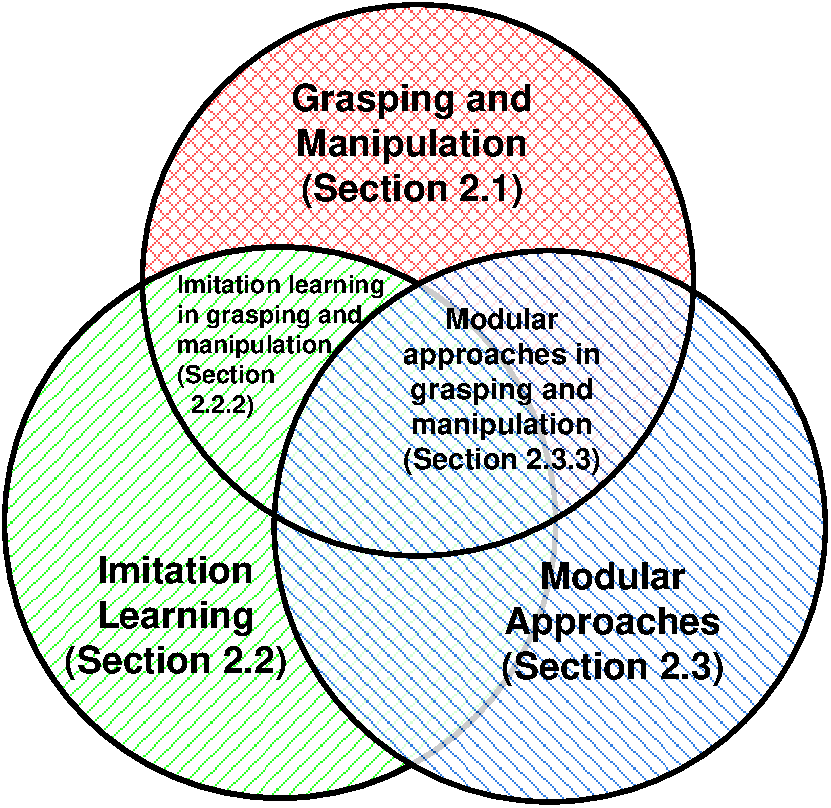
\includegraphics[width=12cm]{./fig_cha2/litreview.pdf}
  \caption{Structure of literature review}
  \label{fig:litreview}
\end{figure}


\section{A review of robot grasping and manipulation}
\label{cha2:sec1}
%TODO: introduction  of grasping and manipulation. What is grasping? What is manipulation?
As discussed in the first chapter, grasping and manipulation problems are important but difficult to solve.
Robot grasping and manipulation research aims to enable robots with a human level ability of handling objects. Grasping and manipulation are usually included in the same research category and are studied by the same robotics community, as they both try to tackle the ``contact tasks'', which  use robot hands (end-effectors) to get physical contacts and interact with target objects.
Robot grasping focuses on how to stabilize the target objects with the support from the robot hand. This involves the problem of where and how to place the hand and fingers to contact the targeted objects. Robot manipulation focuses on delivering the targeted objects from the current state to a desired state, which involves the problem of how to apply forces and torques on the object to achieve the desired state. Besides these two problems, one problem is often discussed by the same community -- the reaching problem. How to move the robot hand to reach the object so that the planned grasps or manipulation strategy can be achieved, for example making contacts in the right places to pick up a box, is the problem studied in reaching. In the later three sections, we will present an overview of these three topics.
%TODO: divide to three sections.
%Reaching: forward and inverse kinematics
%Grasping: analysis and synthesis of closure grasps
%Manipulation: prehensile and nonprehensile

\subsection{Robot grasp planning}
\label{cha2:sec1:planning}
%\label{cha2:sec1:grasping:planing}

% ----- What is grasp planning. Force/form closure -----
The studies of robot grasping have two main categories: geometric based planning and control based execution. The first category studies how to pose the hand and fingers form a stable grasp and the latter studies how to execute a grasp plan and how to make local adjustment to correct a non stable grasp. Early studies of grasping mainly focus on the first category and the second category raise increasing interests in recent years. In this review, we will first look into the planning problem and then move to the execution problem.

Given a robot hand and an object, there are an infinite number of ways to grasp the object. These grasps have different performances and functionalities. Grasp planning is usually formulated as an optimization problem of grasp performance, by finding the contact point locations or robot hand configuration. This technique is call optimal grasp synthesis. The most important criteria in the optimization is the stability of the grasp. In the robot grasping literature, two kinds of ``closure'' are the most extensively used mechanisms for guaranteeing stability: the force-closure and form-closure~\citep{Nguyen87}. A grasp is said to achieve force-closure when the fingers can apply appropriate forces on an object to produce wrenches in any direction~\citep{SalisburyJr1985}. Form-closure is a stronger condition than force closure, which can only be achieved if a grasp is force closure with frictionless contact points~\citep{diziouglu1984mechanics}.

% ---- Grasp quality ----
To measure grasp stability qualitatively, the concept of grasp quality is introduced. Various grasp quality metrics are proposed for different purposes. One important concept involves is the ``grasp wrench space`` that the space of the possible force and torque to be applied by the fingers.
%Starting from the idea of minimizing the sum of the contact forces, \citet{li1988task}, \citet{kirkpatrick1992quantitative} and \citet{ferrari1992planning} propose different measurements of the grasp quality based on the hand wrench space.
The concept of ``task ellipsoid'', which is a geometric representation in the wrench space of the force and torque required in a task, is proposed by \citet{li1988task} to measure how suitable is a grasp for the task: the more overlap between the task ellipsoid and the wrench to be provide by the grasp, the more suitable this grasp is.
\citet{kirkpatrick1992quantitative} refer the grasp quality to the ``efficiency'' of a grasp and define it as the ratio of the largest external wrench that can be balanced by at most one unit force at each contact point. Based on the same principle, \citet{ferrari1992planning} define the quality of a grasp to be the minimum distance from the origin of the wrench space to the boundary of the maximum possible grasp wrench.
\citet{trinkle1992stability} propose a test to measure how far is a grasp away from the form closure.
These metrics are ``object-centric'', i.e. they only consider the contact point locations and the object geometry, while the robot hand configuration is not taken into account. \citet{miller1999examples} take one step further: they use a simulation method to compute the grasp quality of a given object and robot hand configuration. They later develop the physical simulator GraspIt! for grasp quality analysis~\citep{miller2004graspit}. Our work in grasp planing described in Chapter~\ref{cha3} is based on this simulator.

% TODO: Some grasp synthesis methods. Add more.
%Optimal force-closure grasp synthesis is a technique for optimizing the grasping performance by finding the contact point locations.
Optimal force-closure grasp synthesis concerns determining the contact point locations so that the grasp achieves the most desirable performance in resisting external wrench loads.
Based on the grasp quality concept, some approaches optimize an objective function according to a pre-defined quality criterion~\citep{Zhu2003,Zhu04} in the grasp configuration space.
%Some techniques compute optimal force-closure grasps by
%optimizing an objective function according to a pre-defined
%quality criterion~\citep{Zhu04, Zhu03} in the grasp configuration space.
These approaches do not take into account the kinematics of the hand. To bridge this gap, \citet{S.ElKhoury2012} propose a one shot grasp synthesis approach that formulates and solves the problem as a constraint-based optimization.

% ----- Learning and modular methods to tame the dimension -----
Multi-finger grasps usually involve a large number of degrees of freedom.
Searching the grasp space for an optimal grasp requires massive computing time considering the huge number of possible hand configurations. To solve this problem, imitation learning and modular approaches are introduced to constrain the searching space. The relevant literatures are reviewed in Section~\ref{cha2:sec2:grasping-learning} and Section~\ref{cha2:sec3:robotics}

% ----- grasping in cluttered environment -----
The above methods are for static grasp planning that rely on precise and accurate object models. These methods are well suited to controlled industrial environments, for example picking up aligned boxes from the assembly line. However, they are not very applicable for service robots working in human dominated environments. For this reason, in recent years the research has shifted to tackle the problem of maintaining grasp stability in dynamic and cluttered scenes. These studies include handling uncertainty and noise in perceptual data and handling unseen (novel) objects and unforseen situations. To tackle the former problem, one approach is to take the uncertainty and noise into account in the planning and generate robust grasps~\citep{brost1988automatic,zheng2005coping,hsiao2011bayesian}.
\citet{brook2011collaborative} try to handle the uncertainties in object shape estimation by finding a common grasp of the few most possible object shapes.
Besides synthesis, grasping motion is also studied~\citep{,kehoe2012toward}, where the uncertainty is handled by the compliant finger motions. For grasping novel objects, different general object shape representations are proposed. The most studied representations are 2D or 3D local features such as edge, contour and color~\citep{saxena2008robotic,detry2009learning,kroemer2010grasping}, combination of shape primitives~\citep{miller2003automatic,huebner2008minimum,el2010new} and exclusive mathematical representation of the global object surface geometry and topology~\citep{el2013generation,pokorny2013grasp}. Local features allow quick computation of grasps on a sub-part of an object, while global representations allow a global search of good grasps with large computation expenses. Planning grasps for novel objects effectively and robustly remains a challenge.



\subsection{Robot manipulation}
\label{cha2:sec1:manipulation}
%\label{cha2:sec1:grasping:manipulation}

% Current state of art in manipulation

%Different from grasping which aim to stabilize a object, manipulation aim to change the object status, usually its position and orientation, from the current one to the desire one.
Manipulation differs from grasping in that it aims to change the object status, usually its position and orientation, from the current one to the desired one, whereas grasping merely aims to stabilize the object.
This means the problem of manipulation is two-fold: controlling the hand movement to control the object movement.
Studies in manipulation can also be split into two topics: manipulation planning and task execution. The former focuses on planning the hand movement, reasoning how to accomplish a complex task by a sequence of motions and behaviours, while the latter focuses on controlling the object movement, answering the question of how to apply force and torque to deliver a target object to the next desired status. The former problem is mostly addressed by learning from humans and extracting motion primitives from human demonstration, which can be used to build complex behavior for accomplishing a task. We will review those works in Section~\ref{cha2:sec2:grasping-learning} that reviews imitation learning and Section~\ref{cha2:sec3:robotics} that reviews modular approaches. In this section we will concentrate on the latter problem of execution.
%Briefly speaking, there are two directions of approaches: the position and force hybrid control method and the impedance control method.
% Impedance: find a good task impedance.
% force/position hybrid: transition

% open challenge -- to verify your contribution
% why need imitation learning? why need modular?

% Difficulty
%The fundamental difficulty of manipulation is that it requires the robot to adapt to the current situation and tackle sudden changes.
%Manipulation is difficult for that it involves the interaction between robot and the environment.

% TODO: hybrid control
Control methods for manipulation can be roughly divided into two groups: hybrid position$\backslash$force control and impedance control. The hybrid control approaches directly control the force and the position of the robot hand \citep{li1989grasping,yoshikawa1993coordinated}. It specify which few directions to control the force and which directions to control the position and control both of them at the same time. On one hand, this simultaneously direct control of position and force allows a precise control of the hand-environment interaction. On the other hand, it requires a fast reaction to task context changes, e.g. transition between contact and no contact, and a small delay in control may cause large force overshot.


% Impedance control
% TODO: virtual spring
In the contrast, the impedance control method indirectly control the force via defining impedance of the hand~\citep{howard2010transferring,wimbock2012comparison}. Given the desired impedance of a task, we can compute proper motor commands for the robot to accomplish it. Fixed impedance control is limited to simple tasks. In many manipulation tasks such as opening a bottle cap, variable impedance is required: at the beginning we need a large impedance to break the contact between the bottle and the cap, and later we need a small impedance to drive the cap smoothly. For such tasks fixed impedance control will either lead to task failure or cause hardware damage.
However, computing the impedance for a given task involving variable impedance is difficult.
In many cases the impedance is roughly approximated by a linear model, but this is inadequate for non-linear tasks.

Variable impedance can be learnt by humans physically correcting the robot impedance, i.e. wiggling the robot arm, in different stages of the task~\citep{kronander2012online}. For learning manipulation, however, wiggling the robot fingers will interrupt the task and may cause task failure.
%This is feasible for learning robot arm impedance but not for object impedance.
Variable impedance can also be learnt by the Policy Improvement with Path Integrals ($PI^2$) reinforcement learning algorithm, with a task specific cost function~\citep{buchli2011learning}. Designing this cost function requires insight into the task and is usually difficult.

% TODO: rolling and sliding -- difficult
Most of these control methods assume fix point contacts between robot and the environment. In reality, manipulation control always involves rolling and sliding between the contact surfaces. The dynamics of rolling and sliding are analysed in various of studies \citep{howe1988sliding,montana1988kinematics}. These needs to be taken into account in order to rigorously implement the control methods. However, an analytical model of friction that can reliably predict sliding can result in stable analysis of the system dynamics is no yet available \citep{bicchi2001robotic}. This makes the manipulation process hard to predict and requires the robot to adapt to the current situation and tackle sudden changes. This inspires us to learn how human adapt to changing contexts and accomplish manipulation tasks. We presents our study in this direction in the Chapter~\ref{cha4}.



\subsection{Reaching motion planning}
\label{cha2:sec1:reaching}
%\label{cha2:sec1:grasping:reaching}

Reaching motion is another key component in the robot grasping and manipulation problem. Given a computed stable grasp, the question to answer in this study is how to deliver the robot hand to the desired position and form the desired hand posture. This is not a simple path planning problem for the robot arm, but a high dimensional planning problem taking the multiple finger movement into account. On one hand, most studies try to plan a motion to avoid premature collisions between the hand and the object. To this end, the finger movement and the arm movement always need to couple in order to ensure the fingers clutch at the right moment \citep{Shukla2011CDS}, and curve around the object to form the desired grasps \citep{kroemer2011grasping}. To increase the robustness of a grasp, the uncertainty in perception is also taken into account \citep{stulp2011learning}. On the other hand, however, some researches study how to deliberately produce ``premature'' contact with the object.

\citet{chang2010planning} study the human ``pre-grasp'' movements such as sliding a coin to the table edge in order to pick it up, and rotating the handle of a pan to a proper position to grasp it. These methods largely increase the chance of successfully executing a grasp by changing the object's status.

\section{A review of imitation learning}
\label{cha2:sec2}
%\label{cha2:sec2:learning}

This section provides a brief introduction to robot imitation learning and then reviews its applications in robot grasping and manipulation.

\subsection{Robot imitation learning}
\label{cha2:sec2:learning}
Since the first study on robot imitation learning~\citep{friedrich1996robot}, this approach has become one of most popular research areas in robotics. It is considered to be a designer-friendly approach to teach robots new tasks. The aim of imitation learning, also referred to as ``Learn by Demonstration'' (LbD) or ``Program by Demonstration'' (PbD) in some literature, is to enable a robot to learn new skills by observing human demonstrations and then to reuse these skills in similar tasks. In recent years, this approach has been extensively studied~\citep{calinon2007learning,calinon2008robot,dillmann2004teaching,kulic2012incremental} as a promising approach to build robot intelligence.

\subsection{Robot learning grasping and manipulation }
\label{cha2:sec2:grasping-learning}
%\label{cha2:sec4:grasping-learning}

%[El-Khoury and Sahbani, 2010].
%\citet{bekiroglu2011assessing} integral the information of the object shape, approach vector, tactile data and joint configuration to estimate a grasp quality.

% Why need to use learning, benefit?
% ----- reduce complexity -----
As discussed in Section~\ref{cha2:sec1},
conventional grasp and manipulation planning methods suffer from the curse of dimensionality.
Learning techniques have been introduced to avoid the complexity of computing kinematical constraints guaranteeing stable grasps. Briefly speaking, robot grasping has two learning sources: imitation learning from human demonstration and learning from data collected from the simulation.
In imitation learning, some researchers use datagloves for human demonstration. The human hand configuration is then mapped to an artificial hand workspace and the joint angles~\citep{Fischer1998,ekvall2007learning}, or hand preshapes~\citep{Kyota2005, pelossof2004svm, Li07} are learnt. Some other researchers use stereoscopy to track the hand when a demonstrator is performing a grasp~\citep{hueser2006learning} or to match the hand shape to a database of grasp images~\citep{Romero2008}. For long term automatic learning, markerless methods to track human hand and arm movements in the approach and grasp execution are studied~\citep{ekvall2007learning,do2009grasp}. These learning based approaches succeed in taking into account the hand kinematics and generate hand preshapes that are compatible with the object features.
Human grasp postures are usually mapped to robot hand postures in fixed schemes, according to the shape of the object and the type of grasp chosen by human.
The learn from simulation method gets around this mapping step: it directly generates grasps with the robot hand's mechanical constraints. For a given object shape and a robot hand, thousands of grasps are generated in the simulator and later used as training data. \citet{pelossof2004svm} use a discriminative Support Vector Machine model to learn the correlation between the grasp configuration and grasp quality, while \citet{bidan2013grasp} use a generative Gaussian Mixture Model to learn the distribution of force closure grasps. Both models are used to generate new grasps. Grasp training data can also be generated in a real robot platform rather than a simulator~\citep{herzog2014learning}. However, this method is much more time consuming and hence it focuses on finding a way to maximize the use of the grasping experience, i.e. generalizing grasping strategies for novel objects.

To further reduce the complexity of the grasping problem, modular approaches are used. This will be discussed in the Section~\ref{cha2:sec3}.

% ----- uncertainty -----
\textcolor{red}{Besides reducing the complexity of the grasping problem, learning approaches are also used to tackle those common problems that appear in the human environment: uncertainty and noise in perception data, novel objects and unforeseeable situations. Most of these learning approaches study how human handle those situations and imitate the strategies.} \citet{ekvall2007learning,stulp2011learning} study human grasp motion and try to learn how humans choose the approach vector that is robust to noise in pose estimation. Driven by the same idea, the human grasp postures are also studied and mapped to robot hands~\citep{tegin2009demonstration}. Inaccurate execution of a grasp can also cause problems. Human handle this issue by using tactile feedback.
With the recent advances in tactile sensing technology, many attempt to include the tactile sensory data in assessing the grasp stability.
After grasp execution, feedback from tactile sensors provide a more accurate estimation of grasp stability then which provided by vision. This allows grasp correction and can avoid failed lifting of the object caused by instable grasp~\citep{li2014learning}.
\citet{bekiroglu2011assessing} integrate the information of the object shape primitive, approach vector, tactile data and hand joint configuration to estimate a grasp quality.
In the later work, contact point locations are also taken into account~\citep{dang2012learning,dang2014stable}. The support vector machine (SVM) is the most used model in discriminating stable and instable grasps. These tactile based methods are also used to evaluate grasps of novel objects.

% ------ novel object ------
%The tactile feedback based methods usually do not rely on predefined object shapes. Hence these methods can be easily applied to estimate grasp quality for novel objects.
Human's ability in generated grasps for novel objects is also studied and imitated.
\citet{detry2009learning} study the human Early-Cognitive-Vision (ECV), which includes colour and edge information that can be used to describe any objects. These features are associated with appropriate grasps and hence grasps of novel objects with matched features can be generated.
\citet{el2007learning} try to imitate the human mechanism of representing objects by segmenting objects into a set of superquadric shape primitives. The mechanism of a human choosing the grasp component is then learnt by a Neural Network~\citep{el2010new}.



% ----- fast adapt -----
The human environment is dynamic and full of perturbations. These perturbations cannot be foreseen and can only be handled when they happen. A learning approach is also used here to provide methods for quick adaptation. Methods are proposed to simplify the generation of grasps such that a moving object can be caught~\citep{harada2008fast,kim2012,bidan2013grasp}
Besides using visual features, tactile sensors can provide additional useful information not accessible by vision. Many methods for quick adaptation to the actual contact conditions are proposed~\citep{hsiao2010contact,hsiao2011robust,kazemi2012robust,sauser2011iterative,li2014learning}.




% --- Manipulation ---
%%% Compare to analytical solution: more robust, but not guarantee
%%The learning approaches generate give precise contact point locations that guarantee grasp stability. Instead, most of them generate a grasp by less specific specifications such as the approaching vector and pre-grasp postures.
%%At the other hand, these learning approaches usually rely on statistical models. Therefor these approaches do not provide guarantee of the performance of the grasp, even if the plan is execute perfectly. The stability of the planned grasps can only be evaluated after execution. However, for the same reason they tolerate a certain amount of noise and are more robust to errors. Hence, these methods are more suited to human dominate environments.
%%
%%Demonstration based learning has been extensively studied~\citep{calinon2007learning,dillmann2004teaching,kulic2012incremental} as a promising approach to build robot intelligence. %It is essential for the tasks that analytical expression of the system is hard to derive.
%%Learning manipulation tasks is one of the main application of this approach. The physical properties of a manipulation task is hard to express analytically, and as a result the control strategy is hard to derive. Modeling expert's demonstration of strategies has been used as an alternative to the analytical solution.
%%
%%Two major forms of demonstration are used in teaching manipulation tasks: kinematics teaching and tele-operation. In kinesthetic teaching, human directly contact with the robot and guide their movements to accomplish a task~\citep{korkinof2013online,pais2014encoding,pastor2011skill,Miao2014}. The trajectory of movements and contact force are recorded by the robot sensors.
%%% ===== Why not kinematics approach? =====
%%This method is simple and effective but limited in the number of controllable end effectors. While a manipulation task usually involves multifinger movement, a human can kinematically operate one finger with each hand and hence two fingers simultaneously at most. To control multi-finger hands, some researchers use tele-operation~\citep{bernardino2013precision,kondo2008recognition,Fischer98}. This usually relies on data gloves and motion capture system to sense human hand-arm motions. The human motion is mapped to robots to generate motions and interact with the environment. In fine manipulation tasks, the robot platforms are usually restricted to anthropomorphic hands for better mapping. All of these methods provide no direct force feedback to the human demonstrator during manipulation.
%%
%%In some studies, the human demonstrate manipulation tasks with their own bodies~\citep{asfour2008imitation}. With direct interaction with the object the human demonstrator is able to perform the task most naturally and with a more delicate control strategy. The task information captured from these human demonstrations needs to be transferred to robots. Various mapping methods have been proposed~\citep{hueser2006learning,asfour2008imitation,do2011towards,}, while human correction~\citep{calinon2007incremental,sauser2011iterative,romano2011human} and self-correction via learning~\citep{bidan2013robio} are proposed as alternative solutions. In general, how to effectively transfer human skills to robots skill remains a challenge.



%machine learning techniques  to the grasping
%problem. Some researchers use datagloves, map human hand to artificial hand workspace and learn the
%different joint angles~\citep{Fischer98,Ekvall07}, or hand
%preshapes~\citep{Kyota05, Pelossof04, Li07}  in order to perform a grasp. Others use
%stereoscopy to track the demonstrator's hand performing a
%grasp~\citep{Hueser06} or try to recognize its hand shape from a
%database of grasp images~\citep{Romero08}.
%However they focus on different problems, such as telemanipulation~\citep{Fischer98} and human hand tracking~\citep{Hueser06}, rather than real time unattended grasping.
%Other group of researches concentrate on generating a list of grasps for one object~\citep{Kyota05, Pelossof04, Li07, saut2011efficient}.


\section{A review of modular approaches}
\label{cha2:sec3}
%\label{cha2:sec3:modular}
This section first briefly reviews the modular approaches studied in cognitive science and control theory, and then concentrates on modular approaches in robotics.

\subsection{Modular approaches in cognitive science}
\label{cha2:sec3:cognitive}
%\label{cha2:sec3:modular:ai}

% TODO: Modular approach in cognitive science (artificial intelligent and neuroscience), control and robotics
%It has also been shown to be an effective architecture of building intelligent systems~\cite{bryson2004modular,BrysonMcG12}.
% MOSAIC
One typical hypothesis of a modular model in motor control is MOSAIC: the Modular Selection and Identification of Control. It is a paradigm of multiple module control, where each module is composed of a forward model and an inverse model. The forward models are responsible for estimating the task context in real time, and the inverse models are used to generate appropriate motor commands for the context. The inverse models are weighted by the accuracy of the estimations of their corresponding forward models. The final motor command is the linear combination of the commands factored by their weights.

\textcolor{red}{TO BE EXTENDED}

\subsection{Modular approaches in control}
\label{cha2:sec3:control}
%\label{cha2:sec3:modular:control}
%Aim: MMAC is good, useful. Discussed for long. Hard to decide -> learning.

% Adaptive control
The use of modular approaches in control theory is different from that used in AI. As discussed above, in the discipline of AI, modularity is needed when building a large complex versatile system. In the discipline of control theory, on the other hand, modular approaches are used to handle the adaptive control problem, which is usually referred to as multiple model adaptive control (MMAC).
\textcolor{red}{I'm not sure that this last sentence explains what the differences really are between a modular approach in AI and a modular approach in control theory}
%It is method to handel .... problems in adaptive control.
Adaptive control is a control method where the controller changes itself to adapt to the changes in the control condition.
A commonly used example is where the controller of an aeroplane adapts to a reduction in the weight of the jet fuel.
Conventional adaptive control methods rely on state estimation. The controller tries to estimate the changes of the system dynamics and then modulates its control parameters to adapt to the changes. For frequently changing environments, however, the period of modulation of the control parameters may cause a transient error, where strong fluctuations can downgrade the performance and damage the hardware. MMAC is used to reduce the transient error by conducting a fast adaption. A MMAC system is usually composed of several different controllers, each particularly designed for one control condition. During the control process, the environment is monitored in real time and one or more controllers suitable for this environment are activated to generate the control command. When the system encounters a sudden change, it will adapt to it by activating another set of controllers. It does not need to re-optimise the control parameters and hence the transient error is reduced.

MMAC dates back to the 1970s. \citet{athans1977stochastic} use multiple Kalman filters in controlling equilibrium flight, to handle sensor errors and to reconstruct the state variables in different flight conditions. The final adaptive control signal is computed by the linear combination of the control signal generated by each model, weighted by the associated probability. Later, a switching MMAC is proposed and its stability is studied~\citep{fu1986adaptive}.
%Switching was first introduced by Martennson1986
%Morse 1993 study stability
\citet{narendra1994improving} use MMAC to improve the performance of the controller in multiple environments, particularly to reduce the transient error that is caused during the transition of the control parameters from one set of optimal values to another. They later use neural networks to build models for the non linear system~\citep{narendra1995adaptation,narendra1997adaptive}. This controller is implemented in a robot manipulator to follow a predefined trajectory and shows improved performance compared to single model control.

To apply MMAC to a practical control problem, the first step is to design how many modules to use and how to decompose the problem space. For linear plants, this problem is addressed by \citet{anderson2000multiple}. They use the concept of Vinnicombe distance 
\textcolor{red}{need reference to Vinnicombe distance}
to decompose the space. Firstly, an initial random starting point is chosen, where a controller is determined. The controller finds its boundary in the neighborhood where its control is acceptably accurate.
\textcolor{red}{do you mean 'unacceptably', or 'still acceptably'? What defines the boundary condition?}
At the boundary, a new starting point is chosen and a new controller is determined. This process continues until the whole space is covered. Based on this method, \citet{lourenco2006learning} 
\textcolor{red}{citation missing}
propose an approach to recognize the new condition and learn new controls online to adapt. These methods, however, only perform well for learn plants.
\textcolor{red}{learn plants? what?}
How to apply MMAC in nonlinear systems remains a challenge.

In robot control, MMAC has many applications for conducting a task in frequently varying environments. These changing environments can be caused by many factors, such as object interactions. Works on this topic include \citet{petkos2006learning} learning multiple inverse models for controlling robots to follow a trajectory with different workloads on the arm; \citet{nakanishi2013spatio} proposing a time-based switching method for robot systems with variable stiffness actuation to handle the different phases of interaction with the environment; the ``eMOSAIC''~\citep{sugimoto2012emosaic} to bring the MOSAIC from simulation to real robot control. In the last work, the performance of MOSAIC under large observation noise is improved by using an optimal control technique. The method is implemented on the 51 DOF humanoid robot CB-i for a squatting task and a carrying load task. As far as we know, this is the first MMAC implementation for a real robot.

Despite the remarkable theoretical accomplishments and many successful applications of MMAC, its application in controlling service robots is not flourishing. Partly this is because robotics always involves non linear control problems, for which the MMAC has not a principle solution.
\textcolor{red}{need to use another phrase here instead of 'not a principle solution'. Do you mean that MMAC is not the ideal solution for non linear control problems?} 
Also, a MMAC controller itself is difficult to design. Control problems in robotics are highly task specific and the service robots are expected to handle a huge number of tasks.
\textcolor{red}{I have changed 'amount' to 'number' in the sentence above. If the thing we are talking about is continuous we use amount (like for milk), but if it is discrete (like biscuits) then we use number as above. End Lesson :)}
 Hand designing a MMAC for these tasks is not cost effective. %Some of the tasks may needed to be end-user defined, that necessitates a simple user-friendly design scheme.

%But how to modularize is still a problem.
%Anderson 2000 how to decide number of modules for linear plan:
%SMMAC decide when to learn a new module online.
%Predictive control with infinite number of modules.

%Robot:
%Narendra 1995 study robot manipulator
%Sethu with multip phases.
%eMOSAIC
%2012_Design of a grasp force adaptive control system with tactile and slip
%
%
%To handle this problem, the multiple model control is introduced in the 1990's ~\citep{narendra1994improving} and later developed~\citep{narendra1995adaptation,narendra1997adaptive}. This approach is inspired by the local expert model introduced by~\citet{jacobs1991adaptive}. This work propose to use local controllers for different subspaces of the system to improve the control performance.
% Talk about basic idea.  1995 in robot manipulator.

% Talk about developement, 1995 in robot manipulator?

% Read review of adaptive control

%Vinnicombe distance to find number of module?

% Vijarkumar's papers?

% multiple control with mixing. different from local expert?


\subsection{Modular approaches in robotics}
\label{cha2:sec3:robotics}
%\label{cha2:sec3:modular:robotics}
In the previous two sections we list a few applications of the modular approach in robotics from the AI and control prospectives. Modular approaches in robotics go further. In recent years, there have been many studies in the modular approach, especially in robot motion planning, grasp planning and manipulation planning. This is mainly due to the trend to try to move robots from the industrial controlled environment to the human dominated environment, where the robots have to handle dynamic and complex situations. In this section, we will give an overview of modular approaches to motion planning. Applications in grasp planning and manipulation will be reviewed in detail in Section~\ref{cha2:sec5:grasping-modular}.
\textcolor{red}{cross reference missing}
Modularities in robotics always refer to ``primitives'', such as ``object shape primitives'', ``motion primitives'' and ``manipulation primitives''. Among these, the most extensively studied area is motion primitives.
To build a versatile service robot that can work in a human dominated environment and assist a human, high level behaviour planning is required. This means robots need to be equipped with the ability to plan a sequence of movements that fulfil a commanded task, such as ``clean the table'' and ``put the food into the fridge''. The conventional method of motion planning is to search in a high dimensional space formed by the numerous degree of freedoms of the robot. The number of possible solutions to accomplish a task is therefore nearly infinite.

This redundancy is useful. In reality various constraints, such as avoiding obstacles, may be added to the task. Due to the redundancy, we are able to find feasible solutions under multiple task constraints. However, this redundancy also makes planning difficult as the search space is extremely large. One common approach is to carry out optimization for the task with constraints that are mathematically equivalent to the task constraints.
\textcolor{red}{you need to check the last sentence as I have changed it to read properly, but the sense may now be wrong}
The drawback of this optimization approach is that defining a proper cost function and proper constraints for the task is not easy. This requires the robot use to process a certain amount of knowledge in mathematics and mechanism, as well as a deep understanding of the task.
\textcolor{red}{rewrite last sentence as I'm not sure what you are trying to say here}
As an alternative, modular approaches can be used to reduce the search space, without discarding good solutions. To this end, the concept of the motion primitive is introduced into robotics. This is a concept from neuroscience research. Neuroscientists have found evidence to suggest that the vertebrate motor system generates motions by combining a small number of motor primitives~\citep{mussa1994linear,mussa1999modular,bizzi2008combining,grillner2011control}. These show the modularized mechanism running in brains: each motor primitive is one module, the combination of many modules generates the complex behaviour.

This idea inspired roboticists to develop simple motion primitives and use them as substrates to develop complex behaviours. In robot motion planning, motion primitives are defined as the most elementary motions, each of which serves one particular purpose. A common way to generate motion primitives is to extract them from human demonstrations: motion sequences demonstrated by humans are discretized to a sequence of motion primitives. Modularized by the motion primitives, the task planning problem is brought from a huge high dimensional search space to a finite discrete space.
They can be reused in other tasks as functional units. %This motion primitive approach has been studied in many literatures~\ref{}.
\textcolor{red}{I don't think you need this sentence. Its obvious.}

% ----- Model motion primitives -----
A great deal of research literature has discussed the use of motion primitives.
\textcolor{red}{Maybe you should cite some here}
Robot motion primitives are learned from humans. These approaches mainly focus on three problems, which are also the typical problems in a modular approach: how to model the motion primitives, how to extract motion primitives from a complex motion sequence and how to combine them to form a complex behaviour.

In studies of the first problem, many roboticists encode the motion primitives with statistical or analytical models, which can be modulated to some extent by varying the parameters according to the requirements of a certain task. The most used modeling methods for motion primitives are The Hidden Markov Model (HMM), mixture models such as the Gaussian Mixture Model (GMM) and the dynamical systems model represented by a set of non linear differential equations. HMM is used to encode temporal motions~\citep{inamura2004embodied,kulic2008incremental,takano2008integrating,lee2010incremental,bidan2013robio}. For time independent motions, \citet{gribovskaya2010learning,khansari2010imitation} use GMM to model multiple human demonstrations in the state space, while \citet{ijspeert2002movement,Ijspeert2003attractor,schaal2005learning,peters2008reinforcement} use nonlinear differential equations to capture an observed behaviour in an attractor landscape. The later is referred as the Dynamical Movement Primitives (DMP), of which the design principle and roadmap is reviewed in \citep{ijspeert2013dynamical}.

% ----- Segmentation -----
Many of the algorithms mentioned above obtain the motion primitives from manual segmentation of motions. However, it is still not clear to us how many motion primitives we need to compose all the human daily behaviours and what these primitives should be. To obtain these primitives, demonstrating all primitives or manually extracting motion primitives from demonstrations is not practical. Even if a library of motion primitives existed, to learn a complex behaviour from human demonstration, a robot still needs to recover the motion primitives from demonstrated motion sequences. Hence, a general automatic mechanism to extract motion primitives is required.

To this end, segmentation of a motion sequence \citep{takano2006humanoid,Pais2013ID879} and clustering of data \citep{kulic2009online,kulic2012incremental} are the most used techniques. These approaches usually rely on a carefully chosen threshold to decide when to segment and stop clustering. A method is to set boundaries on the kinematic variables such as the velocity: \citet{fod2002automated} segment a sequence when a Zero Velocity Crossing (ZVC) is observed. \citet{takano2006humanoid} perform the segmentation according to the correlation among short motions. They first divide the sequence to a set of short notes. When a new motion is demonstrated, they segment it at the moment that the difference between the predicted next note and actual observed one is larger than a threshold. \citet{kulic2008incremental} use a hierarchical clustering method to extract primitives from human motion sequences. Different cut off parameters are tested to evaluate the trade off effect between facilitating quick group formation and introducing misclassification. \citet{Pais2013ID879} extract the primitives according to the variances of the motions in a few demonstrations for a same task. Many other approaches have been proposed to extract motion primitives according to their task requirements. All of these approaches aim to extract a set of motion primitives that are independent functional units and generalized enough to be reused in many tasks. With these pre-defined motion primitives, online recovery of a sequence of motion primitives is feasible. With the presumption of an existence of a motion primitives library we can reduce the segmentation problem to an online motion recognition problem~\citet{meier2011movement}.
%Approaches in this trend mainly have two directions: algorithms with prior knowledge of the motion primitives and and unsupervised algorithms that do not require prior information. The former direction assume an existence of

% ----- Combine -----
The intention of modelling motion primitives is to use them to help with the motion planning problem. According to the task, the use of the motion primitives can be in the form of selecting, mixing or sequencing. The selecting and mixing are for adaptive behaviour: the robot needs to select one or mix a few motion primitives according to the current task context such that it can finish the task.
%Hence another important trend of study is using primitives to form useful behaviors.
%The ``combination'' has two main forms: selecting and mixing.
Selection can be decided by a pre-learned correlation between the primitives and the task contexts: the highest correlated primitive with the current task context is the one to choose~\citep{takano2006primitive}. On the top of this, \citet{daniel2013learning} use Relative Entropy Policy Search (REPS) to optimize the joint state-action distribution and hence choose the optimal set of parameters for the primitive.
Some others choose the primitive that can result in a system state closest to the desired next system state~\citep{hauser2008using}. A similar idea is used in the mixing method, where more than one motion primitive can be activated at the same time. The weight of each motion primitive is computed to make sure the resulting motion can bring the system to the desired state~\citep{bidan2013robio,sugimoto2012emosaic}. From the human robot interaction perspective, the robot should be able to understand human verbal commands and plan the action. \citet{takano2008integrating} propose a method to associate morpheme words with motion primitives. This potentially enables the robots to understand human commands and plan motion by parsing the sentence.




\subsection{Grasping and manipulation by modular approaches}
\label{cha2:sec3:grasping-modular}
%\label{cha2:sec5:grasping-modular}

Modular approaches in robot grasping and manipulation to reduce the problem complexity. Modularization in grasping and manipulation are mainly done in two approaches: modularize by perception and modularize by action. Perceptual modules are mainly used in planning, while action modules are mainly used in execution.

\paragraph{Modularize by perception}
~\\
The first step of making a plan of grasping and manipulation is observing the object. Most of grasp stability analysis are done based on the shape of an object. In human dominated environment, the possible shapes of objects to grasp and manipulate is infinite. Conventional methods to model these object are only effective in convex models. For highly non-convex shapes, local vision features such as edges and colors are used to generate grasping plans at the local areas. To generate grasp for the whole object, \citet{miller2003automatic} propose a modular approach, i.e. planning grasps by shape primitives. The key idea is to approximate a complex object, e.g. non-convex shape, to a set of shape primitives such as boxes, cylinders and spheres. Planning on these shape primitives is relatively easier or pre-trained. Therefore the complex planning problem is tamed to a set of simple problems. According to different purposes, different shape primitives are proposed. \citet{miller2003automatic} use four primitives including box, cone, cylinder and sphere; \citet{huebner2008minimum} use minimum bounding box to decompose an object and \citet{el2010new} use superquadric as the shape primitive. These methods are based on the complete object point clouds, which may not be fully accessible in the real scenario. Methods to split objects to shape primitives and detect primitives parts are proposed, which mainly exploit the techniques in graphics such as the RANdom SAmple Consensus (RANSAC)~\citep{garcia2009fitting,gallardo2011detection}.
\citet{faria2012extracting} use multiple sensors to track human hand trajectory and tactile data, and hence extract motion primitives and contact primitives from the demonstration. These information is then merged to form a object probabilistic volumetric model, which is decomposed to multiple superquadrics.

\paragraph{Modularize by action}
~\\
The motion primitive concept is also introduced to grasping and manipulation. These differ from the reaching movement primitives discussed in the previous Section~\ref{cha2:sec3:modular:robotics}, where the goal is to reach the targeted points. The grasping and manipulation motion primitives are more task-oriented, i.e. each primitive is associated with a specific impact on the environment, such as getting contact with the object and pushing the object. Therefore in the literature these primitives are sometimes referred to as ``task primitives''. Because of the variety of tasks and their complexity, these task primitives are usually manually defined. Transitions between them are usually decided by contact events that indicate the impacts on the environment~\citep{morrow1997manipulation}. \citet{michelman1994forming} propose the representation of the relationship between task primitives by a finite state machine. \citet{kazemi2012robust} define three task primitives for force compliant grasping of small objects from a table top. The Dynamical Movement Primitives (DMP) mentioned previously, which model desired motion by an attractor landscape, is extended to deal with various problems when executing a grasp. The combination of the DMP and the Early Cognitive Vision Descriptor (ECVD) for grasp planning enable a robot to plan the path of  approach of the hand and the finger to avoid premature contact between finger and object~\citep{kroemer2011grasping}. Taking the object poses distribution into account, a new optimization method of the DMP is proposed to find an approach trajectory that produces robust grasps with object pose uncertainty~\citep{stulp2011learning}. Later simplify version of DMP is used to learn movement goal and hence can quickly change the end point location to adapt to the object shape~\citep{stulp2011learning,stulp2012reinforcement}.
\textcolor{red}{cannot fix last sentence as don't know what you mean - sorry}

A number of frameworks are proposed to model and organize the task primitives. \citet{laaksonen2010embodiment,felip2013manipulation} propose a hierarchical framework to solve the embodiment problem of sharing experience among different robot platforms. This is done by defining task primitives in an abstract layer and an embodiment layer.
\textcolor{red}{defined in two layers then? Should it say ...in both an abstract layer and an embodiment layer}
The former can be translated to the latter. This enables the robot to plan tasks with the higher level abstract primitives, and execute them with the embodiment specific task primitives. To facilitate manipulation motion planning, \citet{barry2013manipulation} use a Rapidly exploring Random Tree (RRT) to sequence motion primitives. \citet{detry2013generalizing} modularize a grasp planning task by two constraints: gripper constraints and task constraints. While the former modules handle grasp stability, the latter modules select grasps from the task requirements.

Besides task-specific motion primitives, modular approaches are also used to tame the complex grasp planning problem. The concept of ``hand synergies'' for example, is a modular approach originating in neurophysiological studies~\citep{santello1998postural,santello2000force}. In this field of study, roboticists try to understand how the human central neural system (CNS) simplifies the grasping strategy and how to mimic this mechanism in robot systems. This concept is used in grip force control \citep{gabiccini2011role} as well as grasp planning \citep{gioioso2013mapping}. Similar to this idea, robot ``Eigen grasps'' have been proposed to study the modularity in robot embodiment. Instead of directly searching for good grasps in the high dimensional configuration space of robotic hands, this space can be reduced by generating a set of grasp starting positions, hand preshapes~\cite{miller2003automatic} or eigengrasps~\cite{Ciocarlie2009} that can then be tested on the object model. Such approaches reduce the dimensionality of the hand configuration space, but doing so implies a corresponding reduction in the accessible hand postures.



%This involve not only the studies of the redundancy in human hand mobility but also the redundancy in human cutaneous and kinaesthetic perception. With the recent rapid development of tactile sensors, robots are equipped with more delicate tactile perception. How collect sensation information from these tactile receptors is also a hot topic in robot synergies. In once word, the study of robot sensorimotor synergies aim to find out the modularity in human muscles, joints, fingers, receptors so as to enable robot working in complex and dynamic system.
% Eigen grasp

%TODO: Problem need to solve in modular approach


%In robot grasping, modularity is also studied. In general, planning a grasp for a multifinger robot hand and a given object shape is a computational expansive task, especially for anthropomorphic robot hand with numerous number of joints. XXXXX~\ref{} proposed the concept of ``eigengrasp'' to simplify the grasp planning problem: three different preshapes of the hand are tested to grasp different objects. Approaching the object with a particular preshape until touching, the hand clutch around the object to form a grasp. XXXXX of objects are successfully grasped by one of the three preshapes. This modular approach reduce the complex grasp planning problem to a simple 3-class classification: one only need to classify with preshapes needs to be used for the target object and decide the approach direction.



%\input{includes/cha2_sec4_grasping-learning}
%\input{includes/cha2_sec5_grasping-modular}
%\section{Imitation learning and modular approaches}
\label{cha2:sec6}

\subsection{Motion primitive}
%\label{cha1:modular:motionprimitive}


%TODO: Hierarchical clustering for motion primitives 





